% ============================================================================
%  Презентация к курсовой работе (защита, ~15 минут, 16 слайдов).
%  Сборка: make slides  (xelatex, из каталога tex/)
%  Текст выступления: speech.md
% ============================================================================
\documentclass[aspectratio=169,11pt]{beamer}

\usepackage{fontspec}
\usepackage{polyglossia}
\setmainlanguage{russian}
\setotherlanguage{english}
\setmainfont{Helvetica Neue}[Ligatures=TeX]
\setsansfont{Helvetica Neue}[Ligatures=TeX]
\newfontfamily\cyrillicfont{Helvetica Neue}[Ligatures=TeX]
\newfontfamily\cyrillicfontsf{Helvetica Neue}[Ligatures=TeX]
\newfontfamily\cyrillicfonttt{Menlo}

\usepackage{amsmath,amssymb,bm}
\usepackage{graphicx}
\usepackage{booktabs}
\usepackage{tikz}
\usetikzlibrary{positioning, arrows.meta, calc}

% ---------- оформление ----------
\usetheme{default}
\setbeamersize{text margin left=9mm, text margin right=9mm}
\definecolor{inkdark}{RGB}{24,40,72}     % тёмно-синий «чернильный»
\definecolor{inkaccent}{RGB}{0,113,134}  % бирюзовый акцент
\definecolor{inkwarm}{RGB}{176,58,46}    % тёплый для контраста/выводов
\setbeamercolor{structure}{fg=inkdark}
\setbeamercolor{frametitle}{fg=white, bg=inkdark}
\setbeamercolor{title}{fg=white}
\setbeamercolor{subtitle}{fg=white!85!inkdark}
\setbeamercolor{author}{fg=white!90!inkdark}
\setbeamercolor{institute}{fg=white!80!inkdark}
\setbeamercolor{date}{fg=white!75!inkdark}
\setbeamercolor{alerted text}{fg=inkwarm}
\setbeamercolor{block title}{fg=white, bg=inkaccent}
\setbeamercolor{block body}{bg=inkaccent!8}
\setbeamerfont{frametitle}{size=\large, series=\bfseries}
\setbeamertemplate{frametitle}{%
  \nointerlineskip
  \begin{beamercolorbox}[wd=\paperwidth, sep=0pt, leftskip=9mm, rightskip=4mm]{frametitle}%
    \vspace{2mm}\insertframetitle\par\vspace{1.5mm}%
  \end{beamercolorbox}}
\setbeamerfont{itemize/enumerate body}{size=\small}
\setbeamerfont{itemize/enumerate subbody}{size=\footnotesize}
\setbeamerfont{block body}{size=\small}
\setbeamerfont{block title}{size=\small, series=\bfseries}
\setbeamertemplate{navigation symbols}{}
\setbeamertemplate{itemize item}{\color{inkaccent}$\blacktriangleright$}
\setbeamertemplate{itemize subitem}{\color{inkaccent!70}$\triangleright$}
% компактные списки: меньше вертикальных отступов
\setlength{\leftmargini}{1.6em}
\addtolength{\itemsep}{-2pt}
\setbeamertemplate{itemize/enumerate body begin}{\setlength{\itemsep}{2pt}}
\setbeamertemplate{footline}{%
  \hbox{\hspace{4mm}\color{inkdark!60}\scriptsize Оптимизация обновления EPD
  \hfill \insertframenumber\,/\,\inserttotalframenumber\hspace{4mm}}\vskip2mm}

\newcommand{\src}[1]{{\tiny\color{black!45}#1}}

\title{\LARGE\bfseries Оптимизация обновления\\электрофоретического дисплея}
\subtitle{\vspace{2mm}курсовая работа}
\author{Хроян Георгий, магистратура, 1 курс}
\institute{Факультет ВМК МГУ имени М.\,В.~Ломоносова}
\date{2026}

\begin{document}

% ---------- 1. Титул ----------
{\setbeamertemplate{footline}{}
\begin{frame}[plain]
  \begin{tikzpicture}[remember picture, overlay]
    \fill[inkdark] (current page.south west) rectangle (current page.north east);
    \node[anchor=south east, inner sep=0, opacity=0.92]
      at ([xshift=-9mm,yshift=11mm]current page.south east)
      {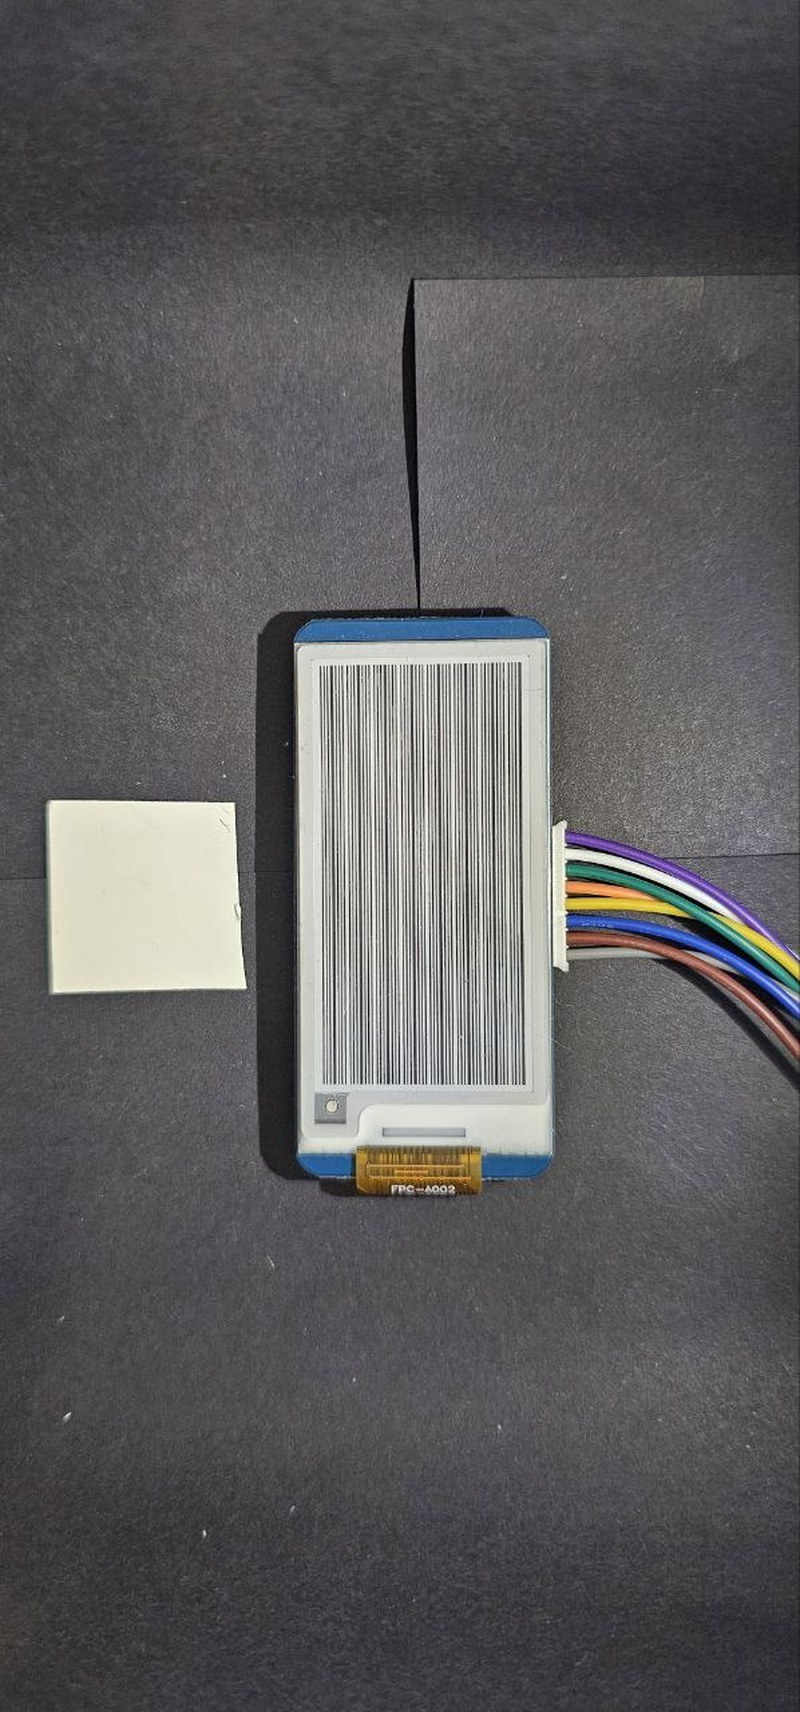
\includegraphics[width=34mm]{figures/raw_photos/epd_checker.jpg}};
    \node[anchor=north west, align=left, text=white, font=\LARGE\bfseries]
      at ([xshift=11mm,yshift=-16mm]current page.north west)
      {Оптимизация обновления\\[1.5mm] электрофоретического дисплея};
    \node[anchor=north west, align=left, text=white!88!inkdark, font=\normalsize]
      at ([xshift=11mm,yshift=-46mm]current page.north west)
      {Хроян Георгий, магистратура, 1~курс};
    \node[anchor=north west, align=left, text=white!75!inkdark, font=\small]
      at ([xshift=11mm,yshift=-54mm]current page.north west)
      {Факультет ВМК МГУ имени М.\,В.~Ломоносова\\[1mm] 2026};
  \end{tikzpicture}
\end{frame}}

% ---------- 2. Проблема ----------
\begin{frame}{Проблема: обновление e-ink стоит дорого}
  \begin{columns}[T]
    \begin{column}{0.58\textwidth}
      \begin{itemize}
        \item EPD: читалки, ценники, IoT-индикаторы~--- сегменты с критичным энергопотреблением
        \item Статичная картинка энергии не требует, \alert{вся цена~--- в моменте обновления}
        \item Обновлением управляет \textbf{waveform}~--- программа импульсов напряжения (LUT контроллера)
        \item Заводские waveform консервативны: длинная осцилляция, запас по температуре
      \end{itemize}
      \vspace{1.5mm}
      \begin{block}{Вопрос работы}
        Сколько можно сэкономить, проектируя waveform \emph{оптимально},~--- и что говорит теория о форме оптимума?
      \end{block}
    \end{column}
    \begin{column}{0.40\textwidth}
      \centering
      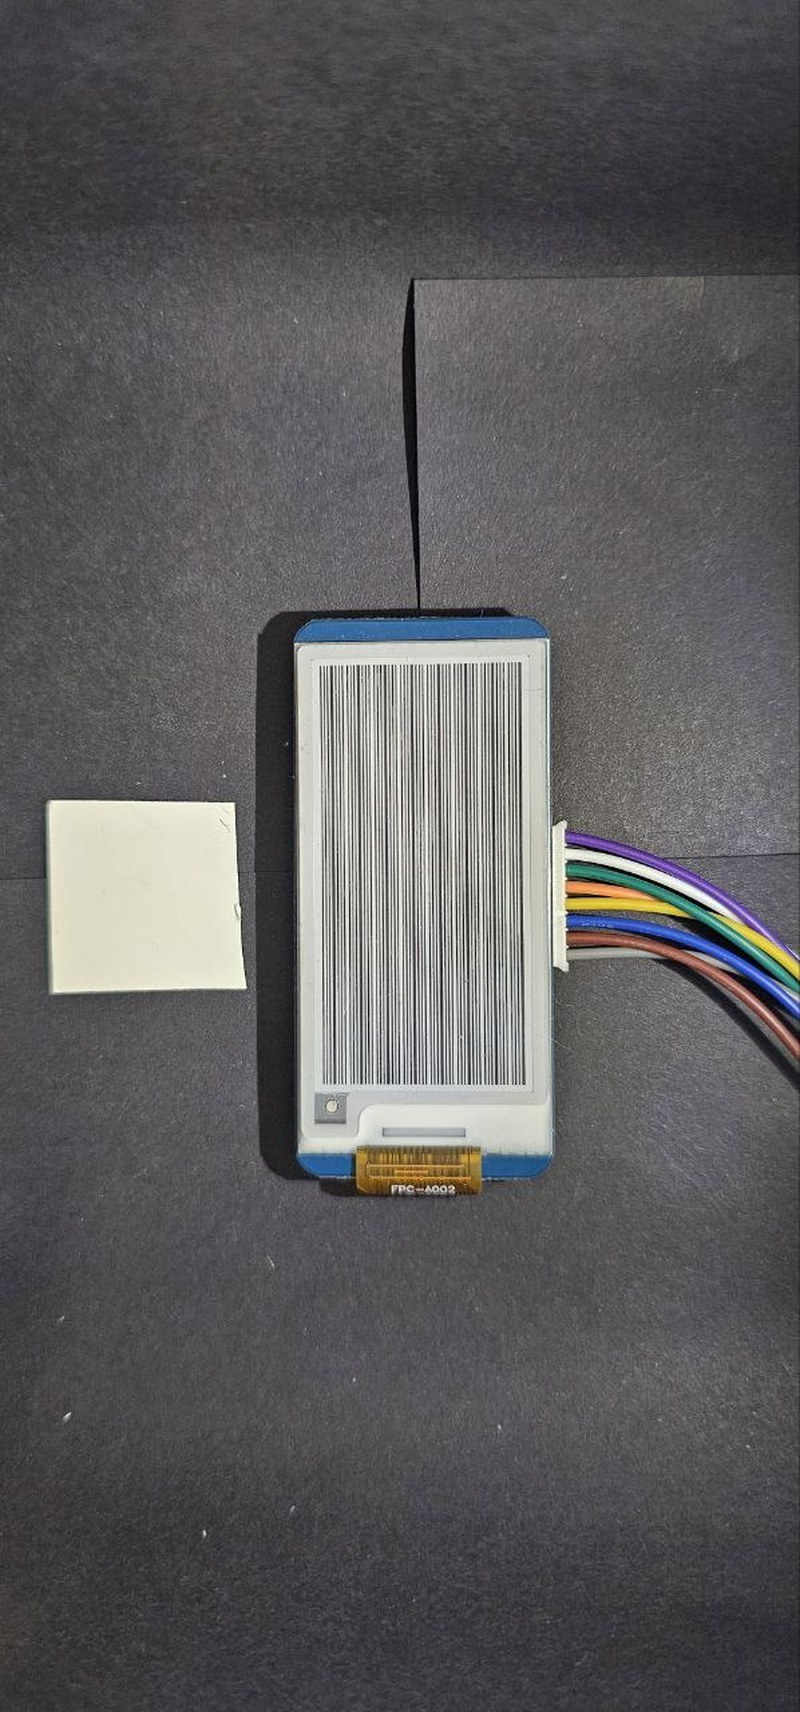
\includegraphics[width=\textwidth]{figures/raw_photos/epd_checker.jpg}\\
      \src{Панель Waveshare 2.13" V4 (SSD1680) на стенде работы}
    \end{column}
  \end{columns}
\end{frame}

% ---------- 3. Цели и задачи ----------
\begin{frame}{Четыре конфликтующие цели и постановка}
  \begin{columns}[T]
    \begin{column}{0.44\textwidth}
      \centering
      \begin{tikzpicture}[font=\footnotesize,
          cell/.style={draw, thick, rounded corners, minimum width=20mm, minimum height=9mm, align=center},
          conf/.style={<->, thick, inkwarm, dashed}]
        \node[cell, fill=blue!12]   (E) at (-1.65, 1.4) {Энергия $E$};
        \node[cell, fill=green!12]  (G) at ( 1.65, 1.4) {Гостинг $G$};
        \node[cell, fill=orange!12] (T) at (-1.65,-1.4) {Скорость $\tau$};
        \node[cell, fill=purple!12] (L) at ( 1.65,-1.4) {Ресурс $L$};
        \draw[conf] (E)--(G); \draw[conf] (E)--(T); \draw[conf] (E)--(L);
        \draw[conf] (G)--(T); \draw[conf] (G)--(L); \draw[conf] (T)--(L);
      \end{tikzpicture}\\[2mm]
      \src{Попарные конфликты целей: единых «правильных весов» нет}
    \end{column}
    \begin{column}{0.54\textwidth}
      \textbf{Цель:} модель и алгоритм оптимизации обновления EPD c Парето-границей компромиссов + проверка на физическом стенде.
      \vspace{1.5mm}
      \textbf{Задачи:}
      \begin{enumerate}\small
        \item каскадная модель: физика $\to$ дискретная задача управления;
        \item структурная теорема о форме оптимальной waveform;
        \item алгоритм построения Парето-границы $(E, G, \tau)$;
        \item аппаратный стенд и измерение энергии/качества;
        \item валидация: полный и частичный режимы, динамический контент.
      \end{enumerate}
    \end{column}
  \end{columns}
\end{frame}

% ---------- 4. Физика ----------
\begin{frame}{Физика панели: главное свойство~--- бистабильность}
  \begin{columns}[T]
    \begin{column}{0.56\textwidth}
      \begin{itemize}
        \item Микрокапсула ($\sim$50 мкм): белые и чёрные заряженные частицы в вязкой жидкости; поле тянет их к электродам
        \item Состояние \textbf{бистабильно}: без напряжения частицы остаются на месте
        \item Следствие (подтверждено экспериментом): \alert{итоговый цвет задаёт последняя фаза драйва}, а не интеграл $\int V\,dt$
        \item Зарядовый баланс $\bigl|\sum V_k T_k\bigr|\le\varepsilon$ нужен \emph{долговечности} панели, а не перемещению
      \end{itemize}
    \end{column}
    \begin{column}{0.42\textwidth}
      \centering
      \begin{tikzpicture}[font=\scriptsize, scale=0.85]
        % капсула
        \draw[thick, fill=yellow!8] (0,0) circle (13mm);
        \fill[white, draw=black!60] (-0.45, 0.75) circle (1.6mm);
        \fill[white, draw=black!60] (0.15, 0.85) circle (1.6mm);
        \fill[white, draw=black!60] (0.62, 0.55) circle (1.6mm);
        \fill[black!85] (-0.55,-0.65) circle (1.6mm);
        \fill[black!85] (0.05,-0.85) circle (1.6mm);
        \fill[black!85] (0.6,-0.6) circle (1.6mm);
        \draw[very thick, inkaccent] (-1.5,1.55)--(1.5,1.55) node[right]{прозрачный электрод};
        \draw[very thick, inkdark] (-1.5,-1.55)--(1.5,-1.55) node[right]{TFT-пиксель};
        \draw[-{Latex}, thick, inkwarm] (-1.85,-0.9)--(-1.85,0.9) node[midway, left]{$\vec E$};
      \end{tikzpicture}\\[1mm]
      \src{Белые частицы у верхнего электрода~--- пиксель белый; смена полярности меняет цвет}
    \end{column}
  \end{columns}
\end{frame}

% ---------- 5. Каскад моделей ----------
\begin{frame}{Каскад моделей: от физики к дискретной задаче}
  \centering
  \begin{tikzpicture}[font=\small,
      lvl/.style={draw, thick, rounded corners, fill=inkaccent!10, minimum width=33mm, minimum height=17mm, align=center},
      arr/.style={-{Latex[length=3mm]}, very thick, inkdark}]
    \node[lvl] (pnp) at (0,0) {\textbf{Континуум}\\ Пуассон--Нернст--\\Планк для $c_\pm(x,t)$};
    \node[lvl] (ode) at (5.1,0) {\textbf{Пиксель}\\ ОДУ центра масс\\ $(\mu^*, \tau^*)$};
    \node[lvl] (disc) at (10.2,0) {\textbf{Дискрет}\\ фазы LUT: $u[k]$, $T_k$\\ $K\le153$ байта};
    \draw[arr] (pnp)--(ode) node[midway, above, font=\scriptsize]{mean-field};
    \draw[arr] (ode)--(disc) node[midway, above, font=\scriptsize]{дискретизация};
  \end{tikzpicture}
  \vspace{4mm}
  \begin{block}{Задача оптимального управления}
    \vspace{-3mm}
    $$\min_{(\mathbf u, \mathbf T)\in \mathcal W_{\mathrm{cb}}(\varepsilon)} \; \alpha E + \beta G + \gamma\tau, \qquad \Bigl|\sum_k V(u[k])\,T_k\Bigr|\le\varepsilon,$$
    \vspace{-4mm}

    управление дискретно: $u[k]\in\mathcal U$~--- аппаратные уровни напряжения SSD1680.
  \end{block}
  \vspace{1mm}
  Энергия и латентность калибруются \emph{на уровне панели}: $E(N)$, $\tau(N)$ по числу активных кадров.
\end{frame}

% ---------- 6. Теория ----------
\begin{frame}{Структурная теория: какова форма оптимума}
  \begin{block}{Теорема 4.1 (структура оптимума)}
    Оптимальная по энергии waveform в классе $\mathcal W_{\mathrm{cb}}(\varepsilon)$~--- релейная (bang-bang), и число активных фаз ограничено:
    $$K_{\mathrm{eff}} \;\le\; d_{\mathrm{state}} + 2 \;=\; 4.$$
  \end{block}
  \begin{block}{Теорема 4.2 (нижняя оценка энергии)}
    Для требуемого изменения отражательной способности $G^{*}$:
    $$E^{*} \;\ge\; K_{\mathrm{lower}}\, G^{*} \qquad \text{(энергетический «пол», дешевле физически нельзя)}.$$
  \end{block}
  \vspace{1mm}
  \begin{itemize}
    \item Доказательство: дискретный принцип максимума Понтрягина (Paruchuri, Chatterjee, 2019) + лемма о знакопеременах показательных сумм
    \item \alert{Практический смысл:} вместо $\sim 10^{300}$ вариантов LUT достаточно перебрать формы с $\le4$ переключениями~--- задача решается точно
  \end{itemize}
\end{frame}

% ---------- 7. Алгоритм ----------
\begin{frame}{Алгоритм: $\varepsilon$-constraint + точный перебор}
  \begin{columns}[T]
    \begin{column}{0.55\textwidth}
      \begin{enumerate}
        \item Сетка ограничений $(\varepsilon_G, \varepsilon_\tau)$ покрывает пространство компромиссов
        \item В каждом узле: $\min E$ при $G\le\varepsilon_G$, $\tau\le\varepsilon_\tau$
        \item Теорема 4.1 сводит узел к перебору малого числа кандидатов ($\le4$ переключений)
        \item Недоминируемые точки $\to$ \textbf{Парето-граница} + waveform для каждой точки
      \end{enumerate}
      \vspace{2mm}
      После калибровки остаются два целочисленных параметра $(T_c, T_d)$: $\sim10^3$ оценок модели, доли секунды на ПК.
    \end{column}
    \begin{column}{0.43\textwidth}
      \begin{block}{Почему не генетика (NSGA-II)}
        Перебор при такой размерности \emph{гарантирует} глобальный оптимум и детерминирован; метаэвристики дают лишь приближение без гарантий.
      \end{block}
      \vspace{2mm}
      \small Тяжёлая оптимизация~--- однократно офлайн; в рантайме только выбор готовой LUT.
    \end{column}
  \end{columns}
\end{frame}

% ---------- 8. Стенд ----------
\begin{frame}{Аппаратный стенд}
  \begin{columns}[T]
    \begin{column}{0.47\textwidth}
      \centering
      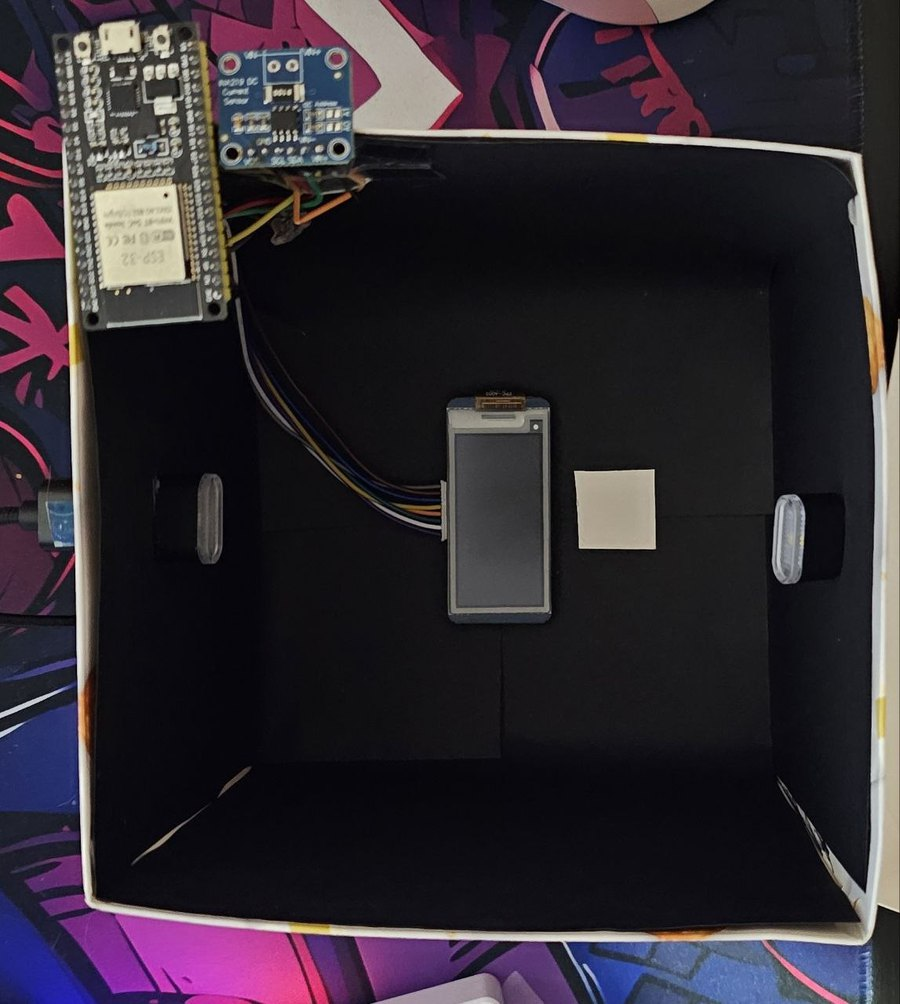
\includegraphics[height=54mm]{figures/raw_photos/stand_overview.jpg}\\
      \src{ESP32 DevKit V1 + Waveshare 2.13" V4 + INA219, камера IP~Webcam над панелью}
    \end{column}
    \begin{column}{0.51\textwidth}
      \begin{itemize}
        \item \textbf{ESP32}: мост USB$\leftrightarrow$SPI, бинарный протокол опкодов; запись кадра, LUT, benchmark-обновления
        \item \textbf{INA219}: питание панели идёт через шунт 0{,}1~Ом~--- ток обновления измеряется напрямую, $E=\int u\,i\,dt$
        \item \textbf{Камера + фотостанд}: контролируемый свет, ROI-выпрямление, нормировка по белому квадрату
        \item Заводские эталоны: \textbf{B0} (полный, OTP) и \textbf{B1} (быстрый, температурный трюк)
      \end{itemize}
    \end{column}
  \end{columns}
\end{frame}

% ---------- 9. Метрика ----------
\begin{frame}{Метрика качества: выбрана эмпирически}
  \begin{columns}[T]
    \begin{column}{0.55\textwidth}
      \begin{itemize}
        \item Семь метрик-кандидатов проверены на монотонных сериях (контраст растёт с длительностью драйва)
        \item Пиксельно-точные (SSIM, региональный контраст) на мелких паттернах дают \alert{отрицательную} корреляцию: субпиксельное рассогласование камеры
        \item Выбрана $\mathrm{otsu\_gap}$~--- разрыв средних яркостей классов Оцу: \emph{не зависит от выравнивания}, $\rho = 0{,}94\ldots1{,}00$ на всех сериях
      \end{itemize}
      \begin{block}{}
        $\mathrm{otsu\_gap} = |\mu_1(t^{*}) - \mu_0(t^{*})|$~--- насколько разделены тёмная и светлая популяции пикселей.
      \end{block}
    \end{column}
    \begin{column}{0.43\textwidth}
      \centering
      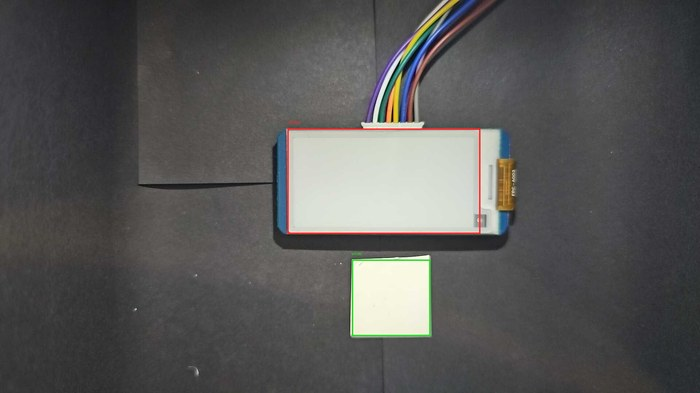
\includegraphics[width=0.92\textwidth]{figures/raw_photos/roi_overlay.jpg}\\
      \src{Кадр камеры: ROI панели и белый калибровочный квадрат}
    \end{column}
  \end{columns}
\end{frame}

% ---------- 10. Калибровка ----------
\begin{frame}{Калибровка панельной модели: $R^2 \approx 1$}
  \begin{columns}[T]
    \begin{column}{0.52\textwidth}
      \centering
      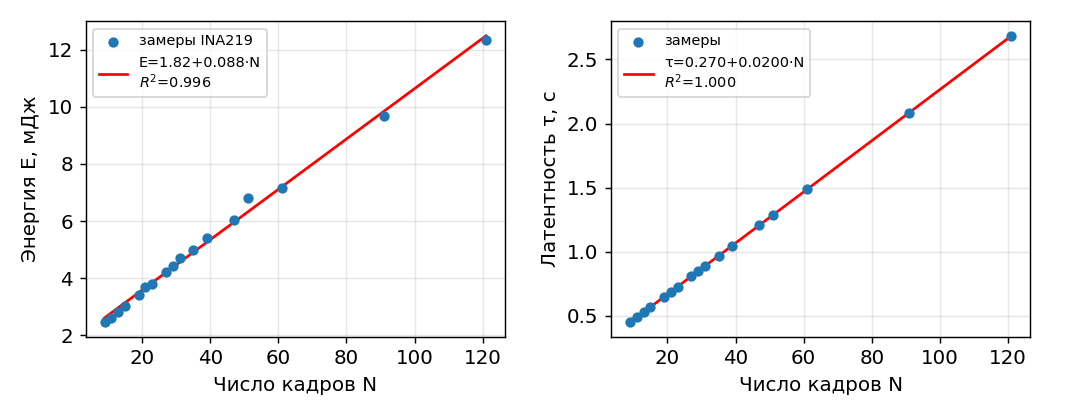
\includegraphics[width=\textwidth]{figures/plots/calib_E_tau.png}\\
      \src{Энергия и латентность линейны по числу кадров $N$}
    \end{column}
    \begin{column}{0.46\textwidth}
      \small
      \[ E(N) = 1{,}82 + 0{,}088\,N \;\text{мДж} \;\; (R^2{=}0{,}996) \]
      \vspace{-5mm}
      \[ \tau(N) = 0{,}27 + 0{,}020\,N \;\text{с} \;\; (R^2{=}1{,}000) \]
      \vspace{-3mm}
      \begin{itemize}
        \item Частота кадров из наклона: $f = 50{,}1$~Гц~--- совпала с допущением модели
        \item Контраст: насыщающаяся модель по фазам ($R^2{=}0{,}978$); осцилляция вчетверо слабее финального драйва
        \item У заводской полной waveform \alert{74\,\% кадров~--- осцилляция}: главный резерв экономии
      \end{itemize}
    \end{column}
  \end{columns}
\end{frame}

% ---------- 11. Главный результат ----------
\begin{frame}{Главный результат: $-50\,\%$ энергии при контрасте B0}
  \begin{columns}[T]
    \begin{column}{0.55\textwidth}
      \small\setlength{\tabcolsep}{3.5pt}
      \begin{tabular}{lccc}
        \toprule
        Waveform & $E$, мДж & $\tau$, с & контраст \\
        \midrule
        Заводская полная (B0) & 11{,}42 & 2{,}27 & 0{,}410 \\
        Заводская быстрая (B1) & 8{,}33 & 1{,}75 & 0{,}385 \\
        \textbf{Наша (равный контраст)} & \textbf{4{,}20} & \textbf{0{,}81} & \textbf{0{,}409} \\
        Наша ($\varepsilon{=}0$, безопасная) & 4{,}71 & 0{,}89 & 0{,}338 \\
        Наша ($\varepsilon$-relaxed) & 3{,}02 & 0{,}57 & 0{,}366 \\
        \bottomrule
      \end{tabular}
      \vspace{2.5mm}
      \begin{itemize}
        \item \alert{$-50\,\%$ энергии и $-54\,\%$ латентности} к B1 при контрасте уровня полного режима B0
        \item Строго DC-сбалансированный режим: $-43\,\%$
        \item Предсказание модели сходится с измерением в пределах 5\,\%
      \end{itemize}
    \end{column}
    \begin{column}{0.43\textwidth}
      \centering
      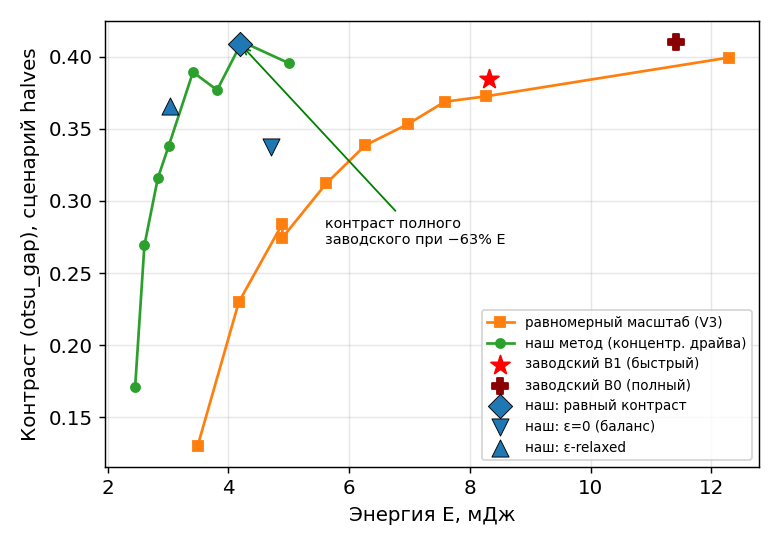
\includegraphics[width=\textwidth]{figures/plots/pareto_energy_contrast.png}\\
      \src{Наш метод доминирует над равномерным масштабированием заводской waveform на всём фронте}
    \end{column}
  \end{columns}
\end{frame}

% ---------- 12. Сценарии ----------
\begin{frame}{Проверка на реалистичном контенте}
  \centering
  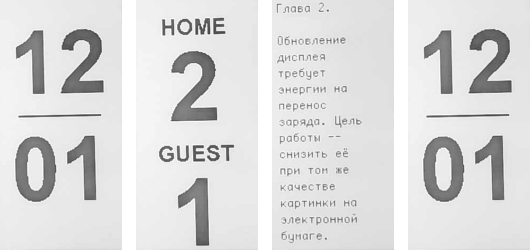
\includegraphics[width=0.58\textwidth]{figures/raw_photos/scenarios_panels.png}\\[1mm]
  \src{Часы, онлайн-табло, страница читалки: наш оптимум против заводского режима}
  \vspace{1mm}
  \begin{itemize}
    \item Визуально неотличимо от заводского полного обновления при вдвое меньшей энергии
    \item Переключение контента без очистки: остаточный след $<1{,}5\,\%$ у обоих~--- экономия не ухудшает ghosting
    \item Циклический тест (8 обновлений): накопления гостинга нет (0{,}099 против 0{,}105 у заводской)
  \end{itemize}
\end{frame}

% ---------- 13. Частичный режим ----------
\begin{frame}{Частичный (безмерцательный) режим}
  \begin{columns}[T]
    \begin{column}{0.50\textwidth}
      \centering
      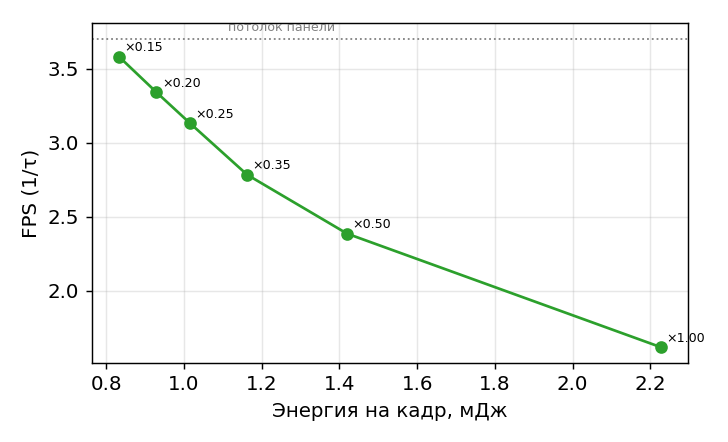
\includegraphics[width=\textwidth]{figures/plots/partial_pareto.png}\\
      \src{Парето частичного режима «энергия на кадр~--- FPS»}
    \end{column}
    \begin{column}{0.48\textwidth}
      \begin{itemize}
        \item Обновляются только изменившиеся пиксели, без вспышки
        \item \textbf{0{,}8--2{,}3 мДж на кадр}~--- в 5--14 раз дешевле полного; до $\approx$3{,}6 обновлений/с
        \item Заводская partial-waveform уже структурно минимальна (одна фаза драйва)~--- наш метод даёт не превосходство, а \emph{выбор рабочих точек} на компромиссе энергия--скорость--контраст
        \item Потолок частоты задаёт среда e-ink ($\tau_0\approx0{,}27$~с накладных), а не TFT-подложка
      \end{itemize}
    \end{column}
  \end{columns}
\end{frame}

% ---------- 14. Видео и интерактив ----------
\begin{frame}{Динамический контент: видео и пинг-понг}
  \begin{columns}[T]
    \begin{column}{0.50\textwidth}
      \centering
      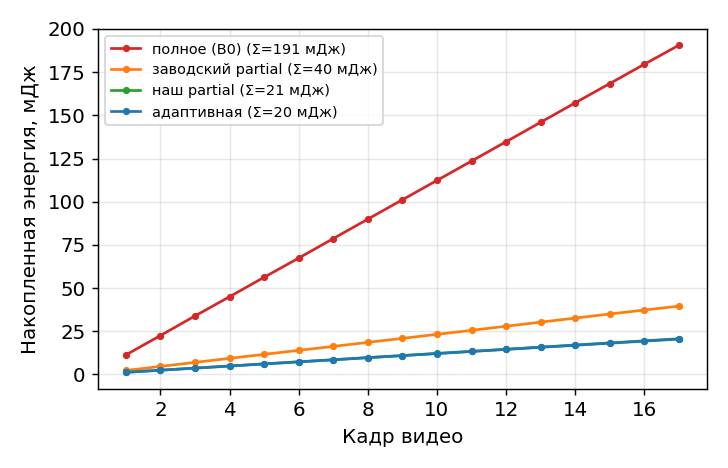
\includegraphics[width=\textwidth]{figures/plots/video_energy.png}\\
      \src{Накопленная энергия за сцену (множество Жюлиа, 17 кадров)}
    \end{column}
    \begin{column}{0.48\textwidth}
      \begin{itemize}
        \item Полное обновление: $\approx$191~мДж за сцену; заводской partial: 40; \alert{наш partial и адаптивная политика: $\approx$21}
        \item Интерактивный пинг-понг: $\approx$3 кадра/с при 1{,}1~мДж против 1{,}6~кадра/с и 2{,}2~мДж у заводского partial
        \item \textbf{Адаптивная политика}: частичные обновления + наш экономный полный сброс по порогу гостинга
      \end{itemize}
      \vspace{1mm}
      \centering
      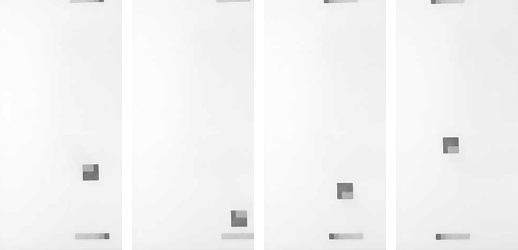
\includegraphics[width=0.50\textwidth]{figures/raw_photos/pong_frames.png}\\
      \src{Кадры авто-игры на панели}
    \end{column}
  \end{columns}
\end{frame}

% ---------- 15. Переносимость и ограничения ----------
\begin{frame}{Переносимость и ограничения}
  \begin{columns}[T]
    \begin{column}{0.50\textwidth}
      \textbf{Что переносится на другие EPD}
      \begin{itemize}
        \item Метод оптимизирует waveform и не зависит от TFT-подложки (a-Si / IGZO / LTPS)
        \item Структурные результаты (релейность, $K_{\mathrm{eff}}\le4$, $\varepsilon$-баланс, partial+сброс) применимы к любой электрофоретической матрице
        \item Панель-зависимы только калибровочные константы~--- перемеряются тем же стендом
      \end{itemize}
    \end{column}
    \begin{column}{0.48\textwidth}
      \textbf{Ограничения честно}
      \begin{itemize}
        \item Одна панель 2.13", чёрно-белый режим
        \item Метрика интегральная ($\mathrm{otsu\_gap}$); пиксельно-точные недоступны из-за оптики
        \item Ресурс при $\varepsilon$-relaxed оценён на коротком горизонте (8 циклов); долгосрочные испытания~--- впереди
        \item Предел FPS задаёт физика среды: единицы герц
      \end{itemize}
    \end{column}
  \end{columns}
\end{frame}

% ---------- 16. Заключение ----------
\begin{frame}{Итоги}
  \begin{enumerate}
    \item Дискретная задача оптимального управления обновлением EPD; доказаны структура bang-bang с $K_{\mathrm{eff}}\le4$ и нижняя оценка $E^{*}\ge K_{\mathrm{lower}}G^{*}$
    \item Стенд (ESP32 + INA219 + фотометрия) и условие исполнения пользовательской waveform на SSD1680
    \item Панельная модель откалибрована с $R^2\approx1$; учтена бистабильность
    \item \alert{Измерено на железе: $-50\,\%$ энергии и $-54\,\%$ латентности при контрасте заводского полного режима}; в DC-безопасном режиме $-43\,\%$
    \item Частичный режим: 0{,}8--2{,}3~мДж/кадр (в 5--14 раз дешевле полного), адаптивная политика для динамики; оптимизация офлайн, в рантайме~--- выбор LUT
  \end{enumerate}
  \vspace{3mm}
  \centering{\large\bfseries\color{inkdark} Спасибо за внимание!}\\[1mm]
  \src{Код, прошивка, данные измерений и сборка~--- в репозитории работы}
\end{frame}

\end{document}
